\documentclass[12pt]{book}
\usepackage[hmargin=0.6in,vmargin=1in]{geometry}
\usepackage{amsmath}
\usepackage{amsthm}
\usepackage[rightcaption]{sidecap}
\usepackage{graphicx}
\usepackage{placeins}
\usepackage{enumerate}
\usepackage{amssymb}
\usepackage{wrapfig}
\usepackage[dvipsnames]{xcolor}
\usepackage{tikz,lipsum,lmodern}
\usepackage[most]{tcolorbox}
\usepackage{hyperref}

\title{Using fancyhdr for Custom Page Header and Footers in a Two-sided Document}

\usepackage{etoolbox}
\makeatletter
% no new page for \chapter
\patchcmd{\chapter}{\if@openright\cleardoublepage\else\clearpage\fi}{}{}{}
% don't change the pagestyle
\patchcmd{\chapter}{\thispagestyle{plain}}{}{}{%
    % example for a warning, 'Package' in text necessary to make TexStudio show it.
    \GenericWarning{(preamble)\@spaces\@spaces\@spaces\@spaces}{Package preamble Warning: patching \string\chapter\space did not work.}}

% allow floats on top of the page with a new chapter
\patchcmd{\chapter}{\global\@topnum\z@}{}{}{}
% if not commented out, first paragraph will be indented
\patchcmd{\chapter}{\@afterindentfalse}{}{}{}
%\makeatother

\usepackage{titlesec}
\titleformat{\chapter}{\normalfont\bfseries\Large}{\thechapter.\quad}{0pt}{}
\titlespacing{\chapter}{0pt}{-5pt}{4pt}% left space, top space, bottom space



\usepackage{fancyhdr}
% Clear off all default fancyhdr headers and footers
\fancyhf{}
\pagestyle{fancy}

\addtolength{\headheight}{\baselineskip}

\fancyhead[L]{\leftmark}
\renewcommand{\chaptermark}[1]{\markboth{\MakeUppercase{#1}}{}}
%\fancyhead[L]{\textbf{\sectiontitle}}
\fancyhead[R]{\sffamily\itshape Lecture Notes on Biophysics}
% Custom text at the left edge of odd pages, and right edge of odd pages.
%\fancyhead[LO,RE]{\sffamily\itshape Fun with fancyhdr}

% Repeat for \fancyfoot if needed, e.g.
% Some decorative symbol at the centre of both odd and even pages
\fancyfoot[L]{\sffamily\itshape Linn Abraham , MGM College of Nursing}
\fancyfoot[C]{\thepage}
\fancyfoot[R]{ June 2020}
% Set this length to 0pt if you don't want any lines!
\renewcommand{\headrulewidth}{2pt}
\pagenumbering{roman}
% Apply the fancy header style


\usepackage{lipsum}
\begin{document}

\title{Sound}
\maketitle
\tableofcontents
\newpage
\setcounter{page}{1}
\graphicspath{ {../} }
\chapter{Applications of Sound}
%\textbf{Applications}:
%\parskip
Some of the application of sound in medical field are :
\begin{itemize}
\item Stethoscope
\item Hearing aids
\item Symbalophone
\item Audiometry
\item Ultrasound scanning
\end{itemize}


\chapter{Hearing}
\begin{itemize}
\item Hearing is the perception of sound.
\item Normal human hearing encompasses frequencies from 20 to 20,000 Hz,.
\item Sounds below 20 Hz are called infrasound, whereas those above 20,000 Hz are ultrasound. Neither is perceived by the ear, although infrasound can sometimes be felt as vibrations.
\item  Other animals have hearing ranges different from that of humans. Dogs can hear sounds as high as 30,000 Hz, whereas bats and dolphins can hear up to 100,000-Hz sounds.
\end{itemize}

\chapter{Vocalisation}
\begin{itemize}
\item In normal breathing,
the vocal cords are relaxed and
air can pass easily through the larynx.

\item A voiced sound is produced when
the cords close off the larynx.

\item As air is exhaled,
pressure builds up behind the cords
and escapes through them.
This reduces the pressure in the back
of the cords.

\item When the pressure is reduced,
the cords again close,
the pressure again increases and
the action is repeated.
\end{itemize}
\begin{figure}[h]
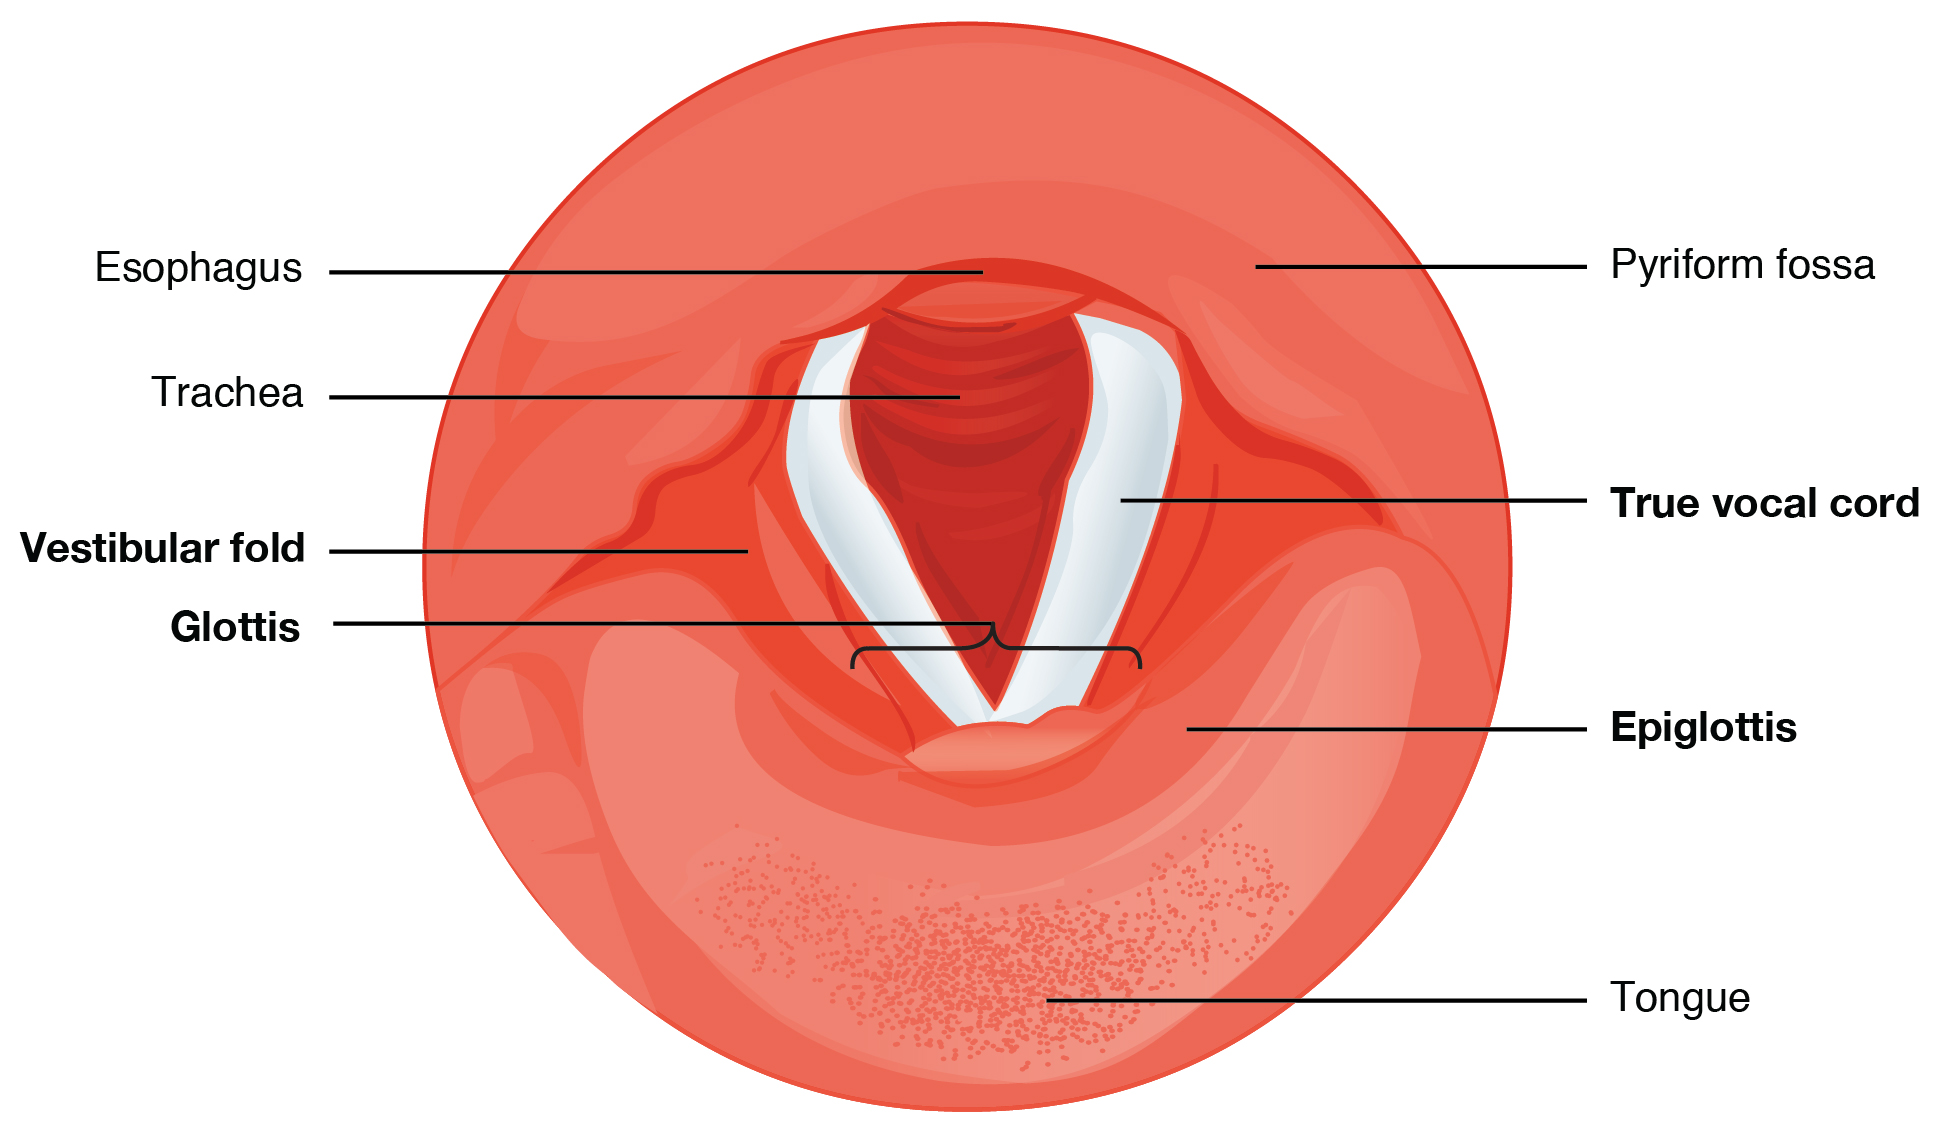
\includegraphics[scale=1]{ vocalcord.jpeg}
\caption{vocal cords}
\end{figure}

\begin{itemize}
\item The character of the voice
is influenced by the tension, thickness
and size of the cords
as well as the size and shape
of the throat, thorax
and para nasal sinuses.

\item This explains why the frequency
of sounds is higher in women and change of voice happens in adolescence
\end{itemize}

\chapter{Hearing}
\begin{figure}[htpb]
    \centering
    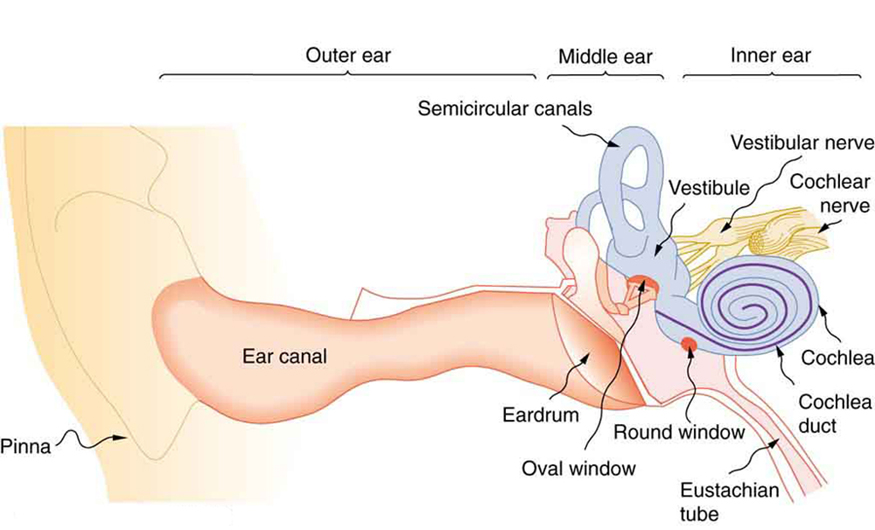
\includegraphics[width=0.8\linewidth]{earanatomy.jpeg}
    \caption{anatomy of the ear}%
    \label{fig:anatomy of the ear.}
\end{figure}
\chapter{Doppler Effect}
\section*{Definition}
“The apparent change in frequency of sound
due to relative motion between the source
of sound and the listener is known as Doppler
effect.”

\section*{Doppler effect in daily life}
\begin{itemize}
\item  Change in sound of a train or ambulance
\item  Speed guns used by police
\item  Doppler effect in light used by astronomers
\item  Doppler scans in hospitals
\end{itemize}


\chapter{Ultrasonic sound}
\section*{Definition}
Ultrasonic sound is sound of a frequency
beyond the highest value in the range of
human audibility

Carries energy that can be absorbed by the medium


\section*{Applications}


\begin{itemize}

\item Provide diagnostic images that complement
those made with x-rays, nuclear medicine, and magnetic
resonance.
\item Heat tissue (diathermy).
\item It is also used to break up gall stones and kidney stones
(lithotripsy)
%\item  experimentally, to destroy tissue by intense heating.
\item Pulverize cancerous tissues in surgical procedure
%\item  Shatter gallstones
%\item Pulversize cancerous tissues
%\item Sonography
%\item Fetal heart monitoring
%\item Echocardiography
%\item Echoencephelograpy
\item Detect motion and determine velocity through the Doppler shift of an echo, known as Doppler-shifted ultrasound.
\end{itemize}

\begin{figure}
\centering
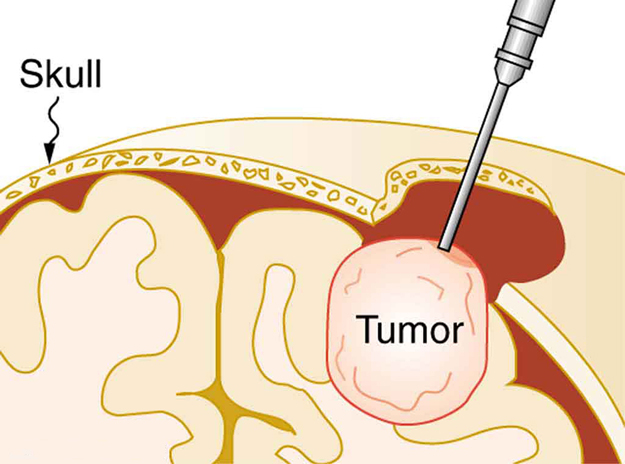
\includegraphics[scale=0.7]{pulverize.jpeg}
\caption{Pulverizing cancerous tissues}
\end{figure}

\section*{Ultrasound Diathermy}
\begin{itemize}
\item Intensities of $10^3$ to $10^4$ W/m2
\item  Applied to injured or overworked muscles
 to relieve pain and improve flexibility.
 “bone burns” and other tissue damage caused by overheating and cavitation,

\end{itemize}

\section*{Ultrasound in medical diagnostics }
\subsection*{Working}
\begin{itemize}
\item When used for imaging, ultrasonic waves are emitted from a transducer, a crystal exhibiting the piezoelectric effect (the expansion and contraction of a substance when a voltage is applied across it, causing a vibration of the crystal).
\item These high-frequency vibrations are transmitted into any tissue in contact with the transducer.
\item  Similarly, if a pressure is applied to the crystal (in the form of a wave reflected off tissue layers), a voltage is produced which can be recorded. The crystal therefore acts as both a transmitter and a receiver of sound.
\item Ultrasound is also partially absorbed by tissue on its path, both on its journey away from the transducer and on its return journey.
\item From the time between when the original signal is sent and when the reflections from various boundaries between media are received, (as well as a measure of the intensity loss of the signal), the nature and position of each boundary between tissues and organs may be deduced.
\end{itemize}
\subsection*{Use}
\begin{itemize}
\item Ultrasound today is commonly used in prenatal care. Such imaging can be used to see if the fetus is developing at a normal rate, and help in the determination of serious problems early in the pregnancy.
\item Ultrasound is also in wide use to image the chambers of the heart and the flow of blood within the beating heart, using the Doppler effect (echocardiology).
\item Many more..
\end{itemize}

\begin{figure}
\centering
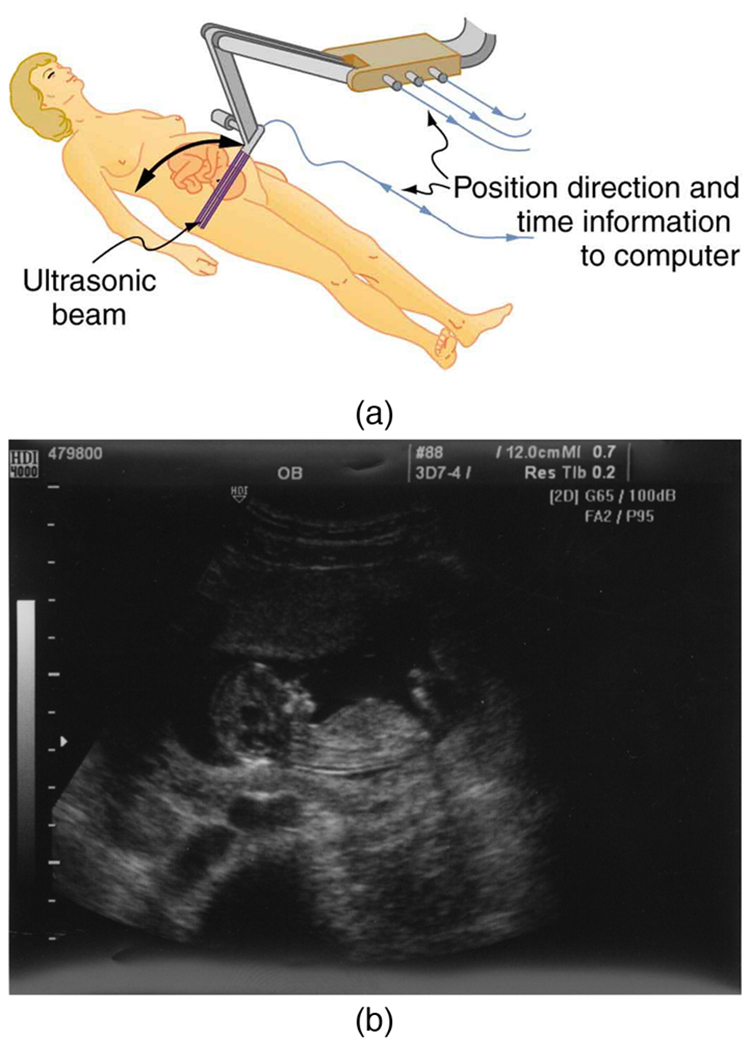
\includegraphics[scale=0.7]{ultrasoundscan.jpeg}
\end{figure}

\section*{Benefits}
\begin{itemize}
\item In addition to shape information, ultrasonic scans can produce density information superior to that found in X-rays, because the intensity of a reflected sound is related to changes in density.
%Sound is most strongly reflected at places where density changes are greatest.
\item The applications of ultrasound in medical diagnostics have produced untold benefits with no known risks.
\item Diagnostic intensities are too low (about  $10^{-2}$W/m2 ) to cause thermal damage.
\item More significantly, ultrasound has been in use for several decades and detailed follow-up studies do not show evidence of ill effects, quite unlike the case for x-rays.

\end{itemize}

\begin{tcolorbox}[colback=red!5!white,colframe=red!50!black,title= Additional Information]
  \begin{description}
      \item[Ultrasound] -  The frequency(or wavelength)  of any wave used for imaging is what limits our resolution for that  particular technique This is the reason why light microscopes have a limit of approximately 500nm and hence are unable to view viruses that are too small. In that case we need electron microscopes. This is also the reason why we do not use audible sound (7cm) but insetead make use  of ultrasonic sound (1.4-0.1mm).

  \end{description}
\end{tcolorbox}

\chapter{Noise}
\section*{Definition}
The common definition of noise is that noise is any unwanted sound.  A better definition of noise is “wrong sound in the
wrong place, at the wrong time”.  The word noise comes from the Latin word nausea meaning seasickness.
\section*{Human health effects of noise pollution}
\begin{itemize}
\item Noise pollution can cause
annoyance and aggression, hypertension, high stress levels, tinnitus,
hearing loss, sleep disturbances, and other harmful effects.
\item Chronic exposure to noise may cause noise-induced hearing loss.
Older males exposed to significant occupational noise demonstrate
significantly reduced hearing sensitivity than their non-exposed peers,
though differences in hearing sensitivity decrease with time and the
two groups are indistinguishable by age 79.
\item High noise levels can contribute to cardiovascular effects and
exposure to moderately high levels during a single eight hour period
causes a statistical rise in blood pressure of five to ten points and
an increase in stress and vasoconstriction leading to the increased
blood pressure noted above as well as to increased incidence of
coronary artery disease.
\end{itemize}

\section*{References}
\begin{enumerate}
\item  Physics of ultrasound (\url{https://openstax.org/books/college-physics/pages/17-7-ultrasound})
\item General ultrasound (\url{https://www.radiologyinfo.org/en/info.cfm?pg=genus})
\item Types of ultrasound (\url{https://stanfordhealthcare.org/medical-tests/u/ultrasound/types.html})
\item Wikipedia (\url{https://en.wikipedia.org/wiki/Medical_ultrasound})
\end{enumerate}

\end{document}
